\documentclass[letterpaper,12pt]{article}
\usepackage[section=]{mathhw}

\usepackage{caption}
\captionsetup[figure]{labelformat=empty}

\usepackage{tikz}
\usetikzlibrary{backgrounds}
\colorlet{fillc}{blue!20}
\tikzstyle{venn} = [
  framed,
  background rectangle/.style={
    thick,
    draw=black,
    fill=white,
  },
  thick,
]

\title{MATH 341 - Extra Point Assignment 2}

\begin{document}

\maketitle

Draw the Venn Diagrams for the following events.

\begin{align*}
  (B \cap A) \cup (A^c \cap B^c) \\
  (B^c \cap A) \cup (A^c \cap B)
\end{align*}

\begin{figure}[!htb]
  \begin{minipage}{.5\linewidth}
    \centering
    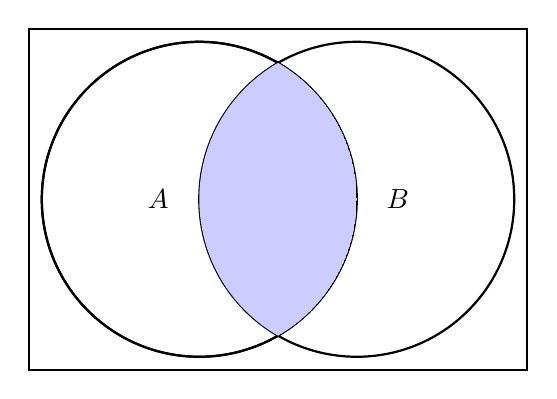
\begin{tikzpicture}[venn]
      \def\radius{2cm}

      \coordinate (A);
      \coordinate[xshift=\radius] (B);

      % Circles
      \draw[fill=white] (A) circle(\radius);
      \draw[fill=white] (B) circle(\radius);
      \draw (A) circle (\radius);

      % Intersection
      \begin{scope}
          \clip (A) circle(\radius);
          \clip (B) circle(\radius);
          \fill[fillc](0,0) circle(\radius);
      \end{scope}

      % Labels
      \node[xshift=-0.5\radius] at (A) {$A$};
      \node[xshift=0.5\radius] at (B) {$B$};
    \end{tikzpicture}
    \captionof{figure}{$B \cap A$}
  \end{minipage}%
  \begin{minipage}{.5\linewidth}
    \centering
    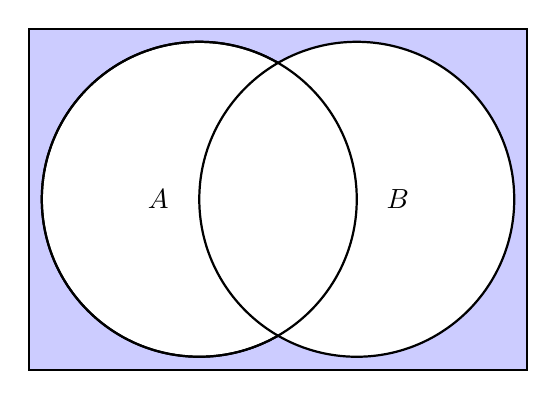
\begin{tikzpicture}[
      venn,
      background rectangle/.append style={
        fill=blue!20
      }
    ]
      \def\radius{2cm}

      \coordinate (A);
      \coordinate[xshift=\radius] (B);

      % Circles
      \draw[fill=white] (A) circle(\radius);
      \draw[fill=white] (B) circle(\radius);
      \draw (A) circle (\radius);

      % Labels
      \node[xshift=-0.5\radius] at (A) {$A$};
      \node[xshift=0.5\radius] at (B) {$B$};
    \end{tikzpicture}
    \captionof{figure}{$A^c \cap B^c$}
  \end{minipage}
  \centering
  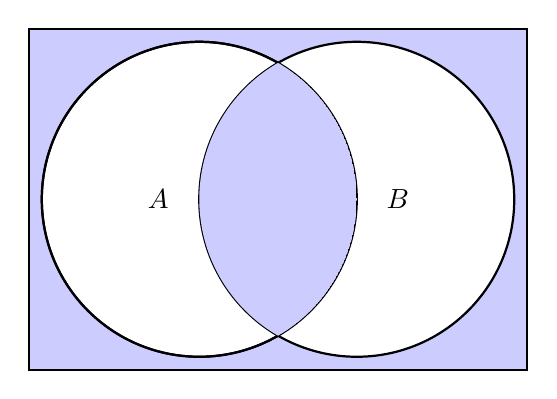
\begin{tikzpicture}[
    venn,
    background rectangle/.append style={
      fill=blue!20
    }
  ]
    \def\radius{2cm}

    \coordinate (A);
    \coordinate[xshift=\radius] (B);

    % Circles
    \draw[fill=white] (A) circle(\radius);
    \draw[fill=white] (B) circle(\radius);
    \draw (A) circle (\radius);

    % Intersection
    \begin{scope}
        \clip (A) circle(\radius);
        \clip (B) circle(\radius);
        \fill[fillc](0,0) circle(\radius);
    \end{scope}

    % Labels
    \node[xshift=-0.5\radius] at (A) {$A$};
    \node[xshift=0.5\radius] at (B) {$B$};
  \end{tikzpicture}
  \captionof{figure}{$(B \cap A) \cup (A^c \cap B^c)$}
\end{figure}

\begin{figure}[!htb]
  \begin{minipage}{.5\linewidth}
    \centering
    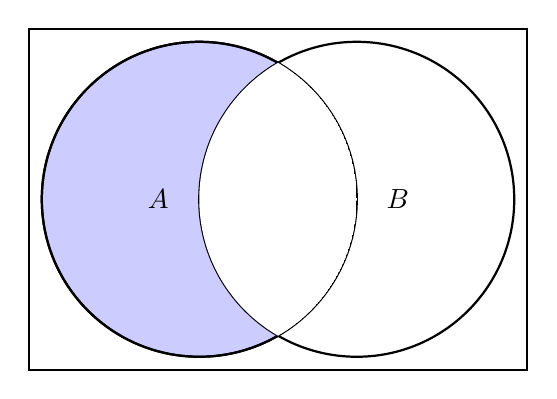
\begin{tikzpicture}[venn]
      \def\radius{2cm}

      \coordinate (A);
      \coordinate[xshift=\radius] (B);

      % Circles
      \draw[fill=fillc] (A) circle(\radius);
      \draw[fill=white] (B) circle(\radius);
      \draw (A) circle (\radius);

      % Intersection
      \begin{scope}
          \clip (A) circle(\radius);
          \clip (B) circle(\radius);
          \fill[white](0,0) circle(\radius);
      \end{scope}

      % Labels
      \node[xshift=-0.5\radius] at (A) {$A$};
      \node[xshift=0.5\radius] at (B) {$B$};
    \end{tikzpicture}
    \captionof{figure}{$B^c \cap A$}
  \end{minipage}%
  \begin{minipage}{.5\linewidth}
    \centering
    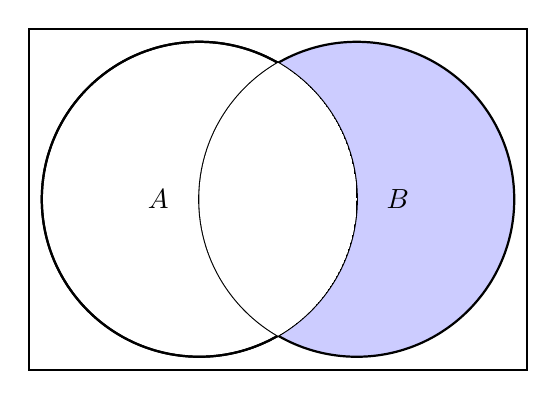
\begin{tikzpicture}[venn]
      \def\radius{2cm}

      \coordinate (A);
      \coordinate[xshift=\radius] (B);

      % Circles
      \draw[fill=white] (A) circle(\radius);
      \draw[fill=fillc] (B) circle(\radius);
      \draw (A) circle (\radius);

      % Intersection
      \begin{scope}
          \clip (A) circle(\radius);
          \clip (B) circle(\radius);
          \fill[white](0,0) circle(\radius);
      \end{scope}

      % Labels
      \node[xshift=-0.5\radius] at (A) {$A$};
      \node[xshift=0.5\radius] at (B) {$B$};
    \end{tikzpicture}
    \captionof{figure}{$A^c \cap B$}
  \end{minipage}
  \centering
  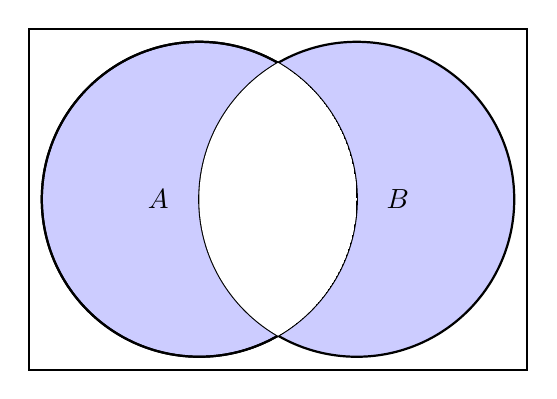
\begin{tikzpicture}[venn]
    \def\radius{2cm}

    \coordinate (A);
    \coordinate[xshift=\radius] (B);

    % Circles
    \draw[fill=fillc] (A) circle(\radius);
    \draw[fill=fillc] (B) circle(\radius);
    \draw (A) circle (\radius);

    % Intersection
    \begin{scope}
        \clip (A) circle(\radius);
        \clip (B) circle(\radius);
        \fill[white](0,0) circle(\radius);
    \end{scope}

    % Labels
    \node[xshift=-0.5\radius] at (A) {$A$};
    \node[xshift=0.5\radius] at (B) {$B$};
  \end{tikzpicture}
  \captionof{figure}{$(B^c \cap A) \cup (A^c \cap B)$}
\end{figure}

\end{document}
